\documentclass[jou,12pt,a4paper]{apa6}\usepackage[]{graphicx}\usepackage[]{color}
%% maxwidth is the original width if it is less than linewidth
%% otherwise use linewidth (to make sure the graphics do not exceed the margin)
\makeatletter
\def\maxwidth{ %
  \ifdim\Gin@nat@width>\linewidth
    \linewidth
  \else
    \Gin@nat@width
  \fi
}
\makeatother

\definecolor{fgcolor}{rgb}{0.345, 0.345, 0.345}
\newcommand{\hlnum}[1]{\textcolor[rgb]{0.686,0.059,0.569}{#1}}%
\newcommand{\hlstr}[1]{\textcolor[rgb]{0.192,0.494,0.8}{#1}}%
\newcommand{\hlcom}[1]{\textcolor[rgb]{0.678,0.584,0.686}{\textit{#1}}}%
\newcommand{\hlopt}[1]{\textcolor[rgb]{0,0,0}{#1}}%
\newcommand{\hlstd}[1]{\textcolor[rgb]{0.345,0.345,0.345}{#1}}%
\newcommand{\hlkwa}[1]{\textcolor[rgb]{0.161,0.373,0.58}{\textbf{#1}}}%
\newcommand{\hlkwb}[1]{\textcolor[rgb]{0.69,0.353,0.396}{#1}}%
\newcommand{\hlkwc}[1]{\textcolor[rgb]{0.333,0.667,0.333}{#1}}%
\newcommand{\hlkwd}[1]{\textcolor[rgb]{0.737,0.353,0.396}{\textbf{#1}}}%

\usepackage{framed}
\makeatletter
\newenvironment{kframe}{%
 \def\at@end@of@kframe{}%
 \ifinner\ifhmode%
  \def\at@end@of@kframe{\end{minipage}}%
  \begin{minipage}{\columnwidth}%
 \fi\fi%
 \def\FrameCommand##1{\hskip\@totalleftmargin \hskip-\fboxsep
 \colorbox{shadecolor}{##1}\hskip-\fboxsep
     % There is no \\@totalrightmargin, so:
     \hskip-\linewidth \hskip-\@totalleftmargin \hskip\columnwidth}%
 \MakeFramed {\advance\hsize-\width
   \@totalleftmargin\z@ \linewidth\hsize
   \@setminipage}}%
 {\par\unskip\endMakeFramed%
 \at@end@of@kframe}
\makeatother

\definecolor{shadecolor}{rgb}{.97, .97, .97}
\definecolor{messagecolor}{rgb}{0, 0, 0}
\definecolor{warningcolor}{rgb}{1, 0, 1}
\definecolor{errorcolor}{rgb}{1, 0, 0}
\newenvironment{knitrout}{}{} % an empty environment to be redefined in TeX

\usepackage{alltt}

%%%%%%%%%%%%%%%%%%%% Loading packages %%%%%%%%%%%%%%%%%%%% 
\usepackage{csquotes}
\usepackage[american]{babel}
\usepackage{amsmath, amssymb, graphicx,gensymb}
\usepackage{fixltx2e} % Misc Latex fixes
\usepackage{url}
\usepackage{threeparttable}
\usepackage[capposition=top]{floatrow}
\usepackage[colorlinks=true,citecolor=blue]{hyperref}
\usepackage{apacite}

%%%%%%%%%%%%%%%%%%%% Set some paramters %%%%%%%%%%%%%%%%%%
\setlength{\parindent}{10mm}
\setlength{\parskip}{0mm}
\graphicspath{ {Figures/} } % path to images

%%%%%%%%%%%%%%%%%%%% Title and such %%%%%%%%%%%%%%%%%%%%%%
\title{\Large Investigating the representational dimensionality and spatial distribution of functional neural networks}
\shorttitle{Dimensionality of functional neural networks}

\author{Lukas Snoek}
\affiliation{University of Amsterdam\\[\baselineskip]
\large Research Master Psychology}
\authornote{Lukas Snoek, student nr. 10126228, University of Amsterdam, Email: lukassnoek@gmail.nl.}

%%%%%%%%%%%%%%%%%%%%%%%%%%%%%%%%%%%%%%%%%%%%%%%%%%%%%%%%%
%  OPTIONAL STUFF  									
%	\leftheader{Snoek}		ONLY IN [jou] MODE			
%	\journal{Journal of Awesomeness}					
%	\volume{2(3)}										
%	\note{version 1}									
%%%%%%%%%%%%%%%%%%%%%%%%%%%%%%%%%%%%%%%%%%%%%%%%%%%%%%%%%

\abstract{In the past decade, cognitive neuroscience witnessed a paradigm shift from functional localization to distributed representations of psychological processes in the brain. Multivariate analyses have been a popular choice to investigate these distributed representations. In the psychological literature, however, the term ``distributeness'' has been used ambiguously and inconsistently, as multivariate representations may be present locally within cortical areas or globally across the entire brain. While local and global multivariate representations are likely encoded at different levels of organisation (across voxels versus across brain areas, respectively), most multivariate analyses are performed without taking the representation's multivariate dimensionality in account. This research proposal aims to investigate the multivariate dimensionality of emotional valence, which is hypothesized to be encoded over brain regions, and contrast this with the locally encoded representations involved in categorical processing. Furthermore, this proposal will exploratively examine how the attribution of valence develops in the brain.}

%%%%%%%%%%%%%%%%%%%% KNITR stuff %%%%%%%%%%%%%%%%%%%%%%%




%%%%%%%%%%%%%%%%%%%% Begin doc! %%%%%%%%%%%%%%%%%%%%
\IfFileExists{upquote.sty}{\usepackage{upquote}}{}
\begin{document}

%%%%%%%%%%%%%%%%%%%% Titlepage! %%%%%%%%%%%%%%%%%%%%

\begin{titlepage}

\newcommand{\HRule}{\rule{\linewidth}{0.5mm}} 
\center 

% Headings
\textsc{\LARGE Graduate School of Psychology}\\[1cm] 
\textsc{\Large University of Amsterdam}\\[1cm]

% Title section
\HRule \\[0.4cm]
{ \huge Research Master's Psychology - MSc. Thesis}\\[0.4cm] 
\HRule \\[1.5cm]
 
% Author section & version/data info
\begin{minipage}{0.4\textwidth}
\begin{flushleft} \large
\emph{Author:}\\
Lukas \textsc{Snoek} 
\end{flushleft}
\end{minipage}
~
\begin{minipage}{0.4\textwidth}
\begin{flushright} \large
\emph{Supervision:} \\
\textsc{Dr. H.S. Scholte} 
\end{flushright}
\end{minipage}\\[1cm]

% Logo

\includegraphics[width=60mm]{uva_logo_inv}\\[1cm] 

% Data
{\large \today}\\[2cm]

\vfill 

\end{titlepage}

%%%%%%%%%%%%%%%%%%%% Start article %%%%%%%%%%%%%%%%%%%%

\maketitle

%%%%%%%%%%%%%%%%%%%% Some notes on knitr %%%%%%%%%%%%%%

%In the code-block below, some data is defined.


%\noindent Inline code output is done as such: max(a).

\section{Introduction}
A key question in the field of cognitive neuroscience is how the brain represents information. A traditional approach in the neuroimaging community is to investigate the representations of psychological concepts and processes as significant activations or deactivations of parts of the brain using functional magnetic resonance imaging (fMRI). This type of analysis is commonly referred to as ``univariate'', because it models each unit of measurement (i.e. voxels) in the brain separately and independently. Effectively, these types of studies aim to localize psychological concepts and functions to particular brain areas. Consequently, researchers implicitly engage in a type of ``neo-phrenology'' in which unique function-structure mappings are pursued \cite{poldrack2010}. For example, the amygdala has become the ``fear area'' \cite{ledoux2003} and a particular part of the fusiform gyrus has become the ``face area'' (and was, in fact, later named the \emph{fusiform face area}).  

In the light of our current understanding of the organization of the human brain, these function-structure mappings are unwarranted. First, for every purportedly selective function-structure mapping, several counter-examples exist \cite{poldrack2010}. The amygdala has, for instance, been implicated in processing stimulus novelty \cite{blackford2010} and the fusiform face area has, for instance, been associated more generally with processing highly familiar objects \cite{tarr2000}. Second, and most importantly, significant \emph{(de)activation} does not imply \emph{representation}; the fact that a brain area activates in response to a certain stimulus does not mean that it represents (processing of) this stimulus.   

In the early 21st century, the cognitive neuroscience community gradually moved from this functional localization perspective to a more network-oriented perspective \cite{sporns2002,barrett2013}. Instead of studying \emph{which} regions (de)activate during a particular psychological process, they started investigating \emph{how} brain areas or a network of brain areas encode and represent this particular process. Rather than treating individual voxels as independent sources of information, researchers realized that by modeling psychological concepts and processes as multivariate representations consisting of interdependent voxels, they could investigate how the brain represents, instead of responds to, information.

One of the first studies to show that the human brain encodes psychological concepts as distributed, multivariate representations was described in the seminal paper by \cite{haxby2001}. They showed that different object categories are represented in a distributed fashion across the ventral visual cortex, regardless of mean activation level. Their approach, for which they used the term Multivariate Pattern Analysis (MVPA), gained popularity quickly as it appeared to provide a more sensitive analysis as opposed to univariate analyses \cite{norman2006,mahmoudi2012} and was consistent with and complemented the emerging network-oriented theoretical framework \cite{bressler2010}. Several new types of multivariate analyses were developed in the succeeding years, including the successful application of machine learning classifiers to distinguish neural representations (e.g. \citeNP{cox2003}) and representational similarity analyses to characterize relations between neural patterns in a continuous, rather than discrete, manner \cite{kriegeskorte2008}. 

Currently, MVPA analyses are widespread in almost all domains of cognitive, affective, and social neuroscience. For example, in vision research, MVPA has been applied to correctly decode stimulus orientation in subregions of V1 \cite{kamitani2005}. At a coarser scale, researchers have shown that it is possible to decode episodic memory traces across the human hippocampus \cite{chadwick2010}. More recently, MVPA has surfaced in the social and affective neuroscience literature, in which it has been used to investigate representations of social and emotional processes. For example, \citeA{kassam2013} has shown that MVPA can be used to decode brain-wide representations of different emotions. It thus seems that MVPA is a useful analysis at different levels of representation, from local (e.g. V1) to global (e.g. emotion networks), and across a range of disciplines.     

% Research gap: what is the problem?
% In thesis: add paragraph about limitation by resolution
Despite the apparent utility of MVPA for different types of research, little is known about how to apply this analysis optimally in different research contexts and disciplines. Currently, most MVPA analyses implicitly assume that representational information is encoded across voxels, meaning that each voxel within a representation carries unique information. While this is likely the case for small-scale, local representations of for example low-level stimulus features such as orientation \cite{kamitani2005} or color \cite{brouwer2009}, several lines of research suggest that with increases in ``globality'' of representations, information from individual voxels becomes less important. In other words, in global representations, information is likely encoded across informational units \emph{larger} than voxels. 

\begin{figure*}[h]
\floatfoot{\textbf{Figure 1}: Three basic types of representations, which vary in spatial distribution (local versus global) and level of encoding (univariate, implying uniformity/redundancy between spatially clustered voxels, versus multivariate, implying encoding of unique information across voxels). Strictly speaking, all patterns are multivariate, but the level of encoding here refers to dimensionality of clusters within global representations.}
\centering
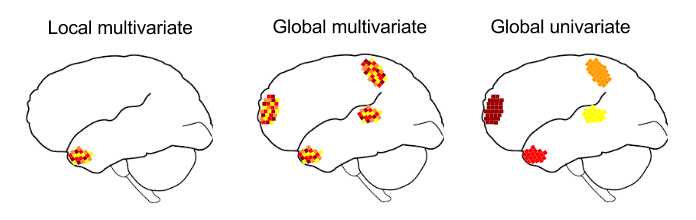
\includegraphics[scale=.55]{spatialDist2}
\end{figure*}

The study by \citeA{brants2011} directly tested this hypothesis by examining the effect of spatial smoothing on voxel patterns within the ventral visual cortex. They showed that spatial smoothing removes information about low-level stimulus features (in this case, spatial frequency) but leaves higher-level category information intact, suggesting different spatial scales for representations of different types of information. Another line of evidence comes from the observation that many MVPA studies in social and affective neuroscience find representations of globally distributed \emph{clusters} of voxels (e.g. \citeNP{oosterwijk2015,kassam2013,corradi2014}). This clustering is unlikely if individual voxels within these clusters indeed carry unique information. This dependence between voxels within clusters has been further supported by the fact that spatial smoothing \cite{oosterwijk2015,kassam2013} does not affect the representation.

This apparent positive association between the globality of representations and the spatial scale of information encoding motivates further investigation on the dimensionality of global versus local representations in the brain. It appears that local representations, e.g. low-level stimulus features such as orientation and color, are indeed encoded across voxels, while more global representations, such as emotion networks, are more likely encoded at a larger scale across clusters of voxels or even entire brain areas. Taken together, it could thus be said that representations may be ``local multivariate'' (i.e. encoded locally across voxels), ``global multivariate'' (i.e. encoded globally across voxels), or ``global univariate'' (i.e. encoded globally across clusters or brain areas). Figure 1 graphically displays these three types of representations. In the current research, we propose to investigate at which level global representations are encoded.

%%%%%%%%%%%%%%%%%%%%
% Mention something about why searchlight mapping is a bad choice when investigating
% large scale networks
%%%%%%%%%%%%%%%%%%%%%%%%%%%%%%%%%%%%%%%%%%%%

%Given the study by \cite{brants2011}, there may be a positive association between the level of information and the spatial scale of information encoding. This would imply that representations of even higher-level psychological processes, such as emotion and motivation, will be represented at even larger spatial scales than object category information. Indeed, one study showed that representations of emotional processes are unaffected by spatial smoothing using a 10 mm kernel \citep{oosterwijk2015}. However, most known studies on higher-level representations such as emotion (e.g. \citealp{kassam2013,baucom2012}, motivation \cite{etzel2015}, and social perception \citep{corradi2014,chavez2015} do not -- a priori -- take into account the spatial scale at which their representations are encoded. The proposed study is aimed at investigating this spatial scale at which higher-level processes are encoded.       

\subsection{Key questions}

In the proposed research, we want to investigate how the level of encoding varies with the globality of representations by contrasting the dimensionality of the representation of category processing, which is known to be (relatively) local multivariate, with the dimensionality of the representation of emotional valence, as emotional valence is known to robustly elicit a brain-wide network of highly clustered, spatially dependent voxels \cite{lindquist2015,chavez2015}.     

% b) Translate the general research question in a clear manner into a specific research question.
To investigate whether emotional valence is encoded as a globally univariate or multivariate representation, we will analyze its representation both as a multivariate pattern of voxels and as a multivariate pattern in which spatial dependence between voxels, i.e. clusters, are taken into account by averaging activity of voxels within clusters. Given these two representations, we will investigate at what spatial scale -- across voxels or across clusters of voxels -- valence information is encoded.  Given the observed strong clustering of spatially dependent voxels in brain-wide representations of higher-level psychological processes, we hypothesize that valence information is encoded across voxel clusters instead of individual voxels. %Moreover, as averaging across spatially dependent voxels increases the pattern's signal-to-noise ratio, we predict that cluster-averaged valence representations can be better classified than the original voxel-level valence representations (as demonstrated by \citealp{brants2011}).  

Furthermore, as an exploratory addition to this research, we want to examine how and where the representation of valence develops in the brain over time. Questions that will be addressed, but do not bear any a priori hypotheses, include whether valence is represented as a global functional network from the beginning or gradually develop in a local-to-global fashion, and at what rate valence develops. Together with this study's confirmatory part, we hope to contribute to a better understanding of the level of encoding of higher-level psychological processes as well as to show how the development of these representations can be investigated over time.\\

\bibliographystyle{apacite}
\bibliography{refs}

\end{document}
